%=== CHAPTER FOUR (4) ===
%=== Test and Experiments ===

\chapter{Experiments}
\begin{spacing}{1.5}
\setlength{\parskip}{0.3in}
\section{Dataset}
To the best of our knowledge, there is currently no dataset for studies of skin blemish modification and fading. We thus adopted a self-collected dataset for our research, development, and testing. The images within the dataset were acquired by two clinical imaging systems (Visia CR4 and OLE both developed by Canfield Scientific). They were cross-polarized and color-calibrated and had a minimum resolution of 3700$\times$5600. The dataset consists of 342 subjects within the age range of 18 to 45 years, encompassing multi-ethnic consumers with skin tones ranging from dark to tan. The collection period lasted for a duration of up to 3 months during the Summer season with a time step of one week.

In our simulation, we input images of Week 0 and adjust the parameters of the obtained model to simulate the change of the blemishes in the following weeks. As shown in Figure\ref{fig:forward}, we labelled the input as \textit{Week 0} and the images for the next few weeks as \textit{+n W}.

\section{Experiment Setup}
In this study, we have carried out extensive blemish change simulation experiments to evaluate the algorithm's effectiveness. We fitted each pigmentation with 3 Gaussian functions summation and set $\sigma=10$ for the skin texture layer separation filter. We mainly focused on the relative concentration changes of the pigmentation, and we conducted a series of simulations based on tuning the concentration parameter after successfully fitting pigmentations.

We select the inpainting mode of \textbf{Stable Diffusion}(SD)\cite{rombach2021highresolution} and \textbf{Adobe Photoshop}(PS)'s inpainting tool\cite{adobephotoshop} for comparison as baseline models. The former, a top-performing deep learning model, represents the "latent space editing" method discussed. We control the intensity of blemish removal by adjusting the denoising level. The latter, a common image editing software, represents the "pixel space editing" method. Here, we adjust the degree of blemish removal by altering layer blending opacity.

\subsection{Objective Evaluation}
To objectively evaluate image modifications, we apply the Fréchet Inception Distance (FID). FID is a common tool for assessing GANs and similar image-generating models. It uses the Inception V3\cite{DBLP:conf/cvpr/SzegedyVISW16} model to derive the mean and covariance matrix of feature vectors from both authentic and generated image collections. Then, it calculates the Fréchet distance between these statistical groups. This distance gauges the variation between two multi-dimensional Gaussian distributions. Generated images resembling real images more closely have lower FID scores, while higher scores show a bigger divergence. Formally, the FID score is denoted as:

\subsection{Subjective Evaluation}
To subjectively evaluated the performance of the proposed facial skin blemish simulation algorithm, a visual perception study is conducted. The aim was to comprehensively evaluate whether the algorithm could produce authentic and believable blemish changes and to analyses whether there are biases in certain attributes of the skin, such as skin color or age. A group of 500 panellists were joined for this study, whose age groups were divided into three categories: 19-25; 26-34; and 35-45, covering various ethnicities including Caucasians, African-Americans, Asians, Hispanics, and others, as shown in Figure \ref{fig:metadata}.
\begin{figure}[t!]
    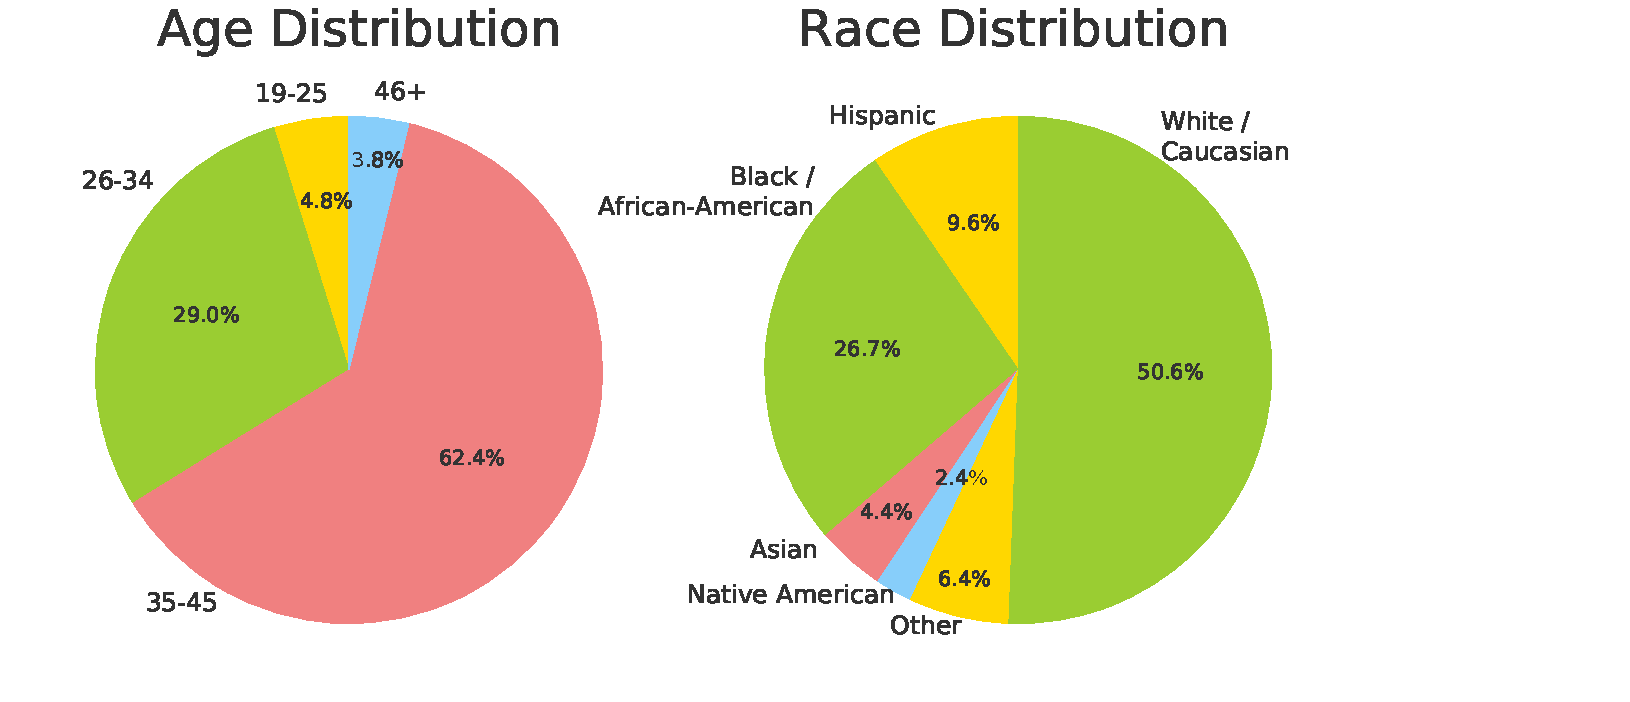
\includegraphics[width=0.95\columnwidth]{Chapter4/metadata.pdf}
    \caption{Metadata of panellists. The test population covers people from 19 to 45 years old, multiple races, and multiple skin tones}
    \label{fig:metadata}
\end{figure} 
In our survey, each panellist answered 10 questions. The question we asked was \textit{You will see a series of patches from face images. Some images have been modified so that some spots (acne or pigmentations) on the skin have been reduced/removed by computer software. You are invited to assess how confident you are that the image you see has been modified.} The answer options were set as:
\begin{itemize}
    \item Very Confident HAS been altered (-2)
    \item Confident HAS been altered (-1)
    \item Not Sure (0)
    \item Confident has NOT been altered (+1)
    \item Very Confident has NOT been altered (+2)
\end{itemize}

In the survey, 48 images (24 simulated through our algorithm and 24 unaltered images) were shown to the panellists one image at a time. When the score ranged from 0 to +2, we considered the respondents to be affirming the image as "real" rather than modified.

%=== END OF CHAPTER FOUR ===
\end{spacing}
\newpage
